\section{Background}
The double pendulum is a classic system used in Dynamics courses everywhere.  Over the course of the class, we have solved equations of motion and simulated models of both simple (massless bars) and compound (bars with mass) planar double pendulums using Newton's Second Law and Euler's Equations.  In this project, we hope to extend the double pendulum system we have studied so well into a triple compound pendulum with damping at the joints.  The experimental system we are trying to model is shown in figure \ref{expsetup}.  The bars of the pendulum have significant mass, requiring the inclusion of rotational dynamics in the system. Furthermore, the system has been observed to damp significantly over time. To solve these equations of motion, we will explore the use of Lagrangian Mechanics for non-conservative systems and will solve for equations of motion.  We will create a numerical simulation for the system in order to explore our equations of motion and will validate them by comparison to experimental data from a real planar triple pendulum system. 

\begin{figure}[H]
\centering
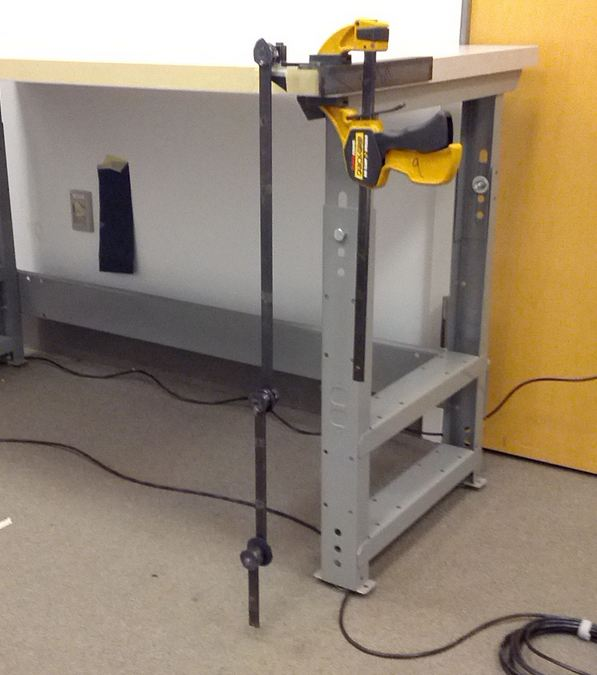
\includegraphics[scale=0.3]{testsetup.JPG}
\caption{Experimental Test Setup.}
\label{expsetup}
\end{figure} 

The system in question is considerably more complicated than the traditional double pendulum studied. The bars of the pendulum have significant mass, that is, the pendulum is not a set of bobs joined by strings, but a set or bars with joints. Furthermore, the joints are not neccesarily frictionless. A picture of the experimental setup we hope to model is shown in Figure \ref{expsetup}.

The tools necessary to complete this modeling came almost entirely from Dynamics lectures.  Additional reading$^{1,4}$, however, was done on use of Lagrangian energy methods for nonconservative systems. Numerous sources$^{2,3}$ present a derivation of the equations of motion of a double pendulum using energy methods. However, we were unable to find any sources which derived the equations of motion of a triple pendulum. Several sources$^{5}$ show simulations of triple pendulums: we used these to validate our model.

